\section{Resultate und Diskussion}

Die berechneten Werte sind  als  Tabelle  und  grafisch  zusammengefasst  (siehe
Tabelle \ref{tab:zusammenfassung} und  Abbildung \ref{fig:einzelmessungen}).

\begin{table}[ht!]
    \begin{center}
        \caption{Zusammenfassung der errechneten Werte}
        \label{tab:zusammenfassung}
        \begin{tabular}{lrrr}
            \toprule
                                    & Ohne Kalibration                                    & Mit Kalibration                                   \\
            \midrule
            Remo Suter              & $(294.52 \pm 10.37)\cdot 10^6\textrm{m}/\textrm{s}$  & $(297.82 \pm 10.49)\cdot 10^6\textrm{m}/\textrm{s}$  \\
            Alex Murray             & $(282.79 \pm 6.65) \cdot 10^6\textrm{m}/\textrm{s}$  & $(284.22 \pm 6.75)\cdot 10^6\textrm{m}/\textrm{s}$  \\
            \midrule
            Gewichtete Mittelwerte  & $(286.21 \pm 5.60)\cdot 10^6\textrm{m}/\textrm{s}$   & $(288.20 \pm 5.67)\cdot 10^6\textrm{m}/\textrm{s}$  \\
            \bottomrule
        \end{tabular}
    \end{center}
\end{table}

Es ist klar zu sehen dass Herr Suter genauer gemessen hat als Herr Murray, weil
die Sicherheit bei allen  Messungen kleiner ist. Die Kalibrationsmessung hat die
Sicherheit  nicht wesentlich verbessern k\"onnen, jedoch hat sie  die  Resultate
n\"aher am ``wahren Wert'', sprich, Literaturwert verschieben  k\"onnen,  wie in
der Abbildung \ref{fig:einzelmessungen} sch\"on zu sehen ist.

\begin{figure}[ht!]
    \centering
    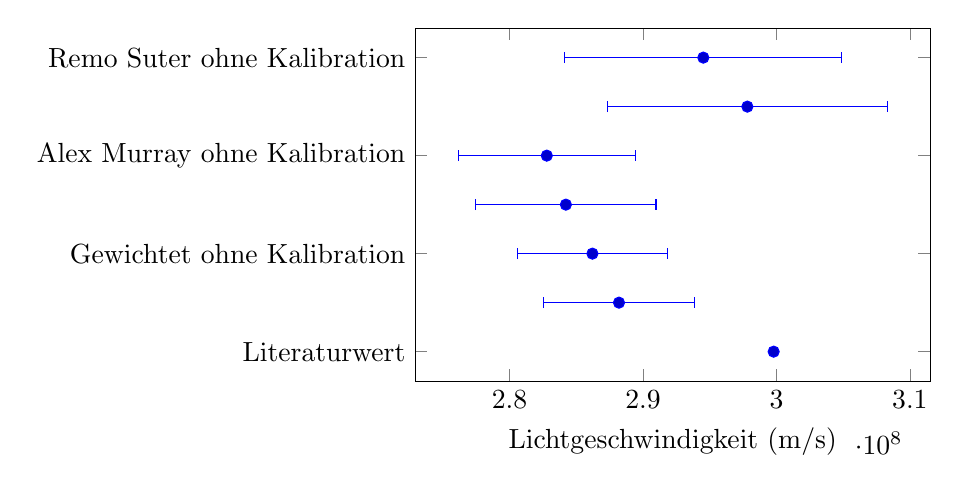
\begin{tikzpicture}
        \begin{axis}[
            width=.67\textwidth,
            height=.5\textwidth,
            xlabel = {Lichtgeschwindigkeit (m/s)},
            symbolic y coords = {Literaturwert,
                                 Gewichtet mit Kalibration,
                                 Gewichtet ohne Kalibration,
                                 Alex Murray mit Kalibration,
                                 Alex Murray ohne Kalibration,
                                 Remo Suter mit Kalibration,
                                 Remo Suter ohne Kalibration},
        ]
        \addplot+[
            only marks,error bars/.cd,
            x dir=both,x explicit,
            error bar style={line width=0.5pt},
            ]
        coordinates {
            (299790000,Literaturwert)
            (286210000,Gewichtet ohne Kalibration)          +- (5600000,0)
            (288200000,Gewichtet mit Kalibration)           +- (5670000,0)
            (284220000,Alex Murray mit Kalibration)         +- (6750000,0)
            (282790000,Alex Murray ohne Kalibration)        +- (6650000,0)
            (297820000,Remo Suter mit Kalibration)          +- (10490000,0)
            (294520000,Remo Suter ohne Kalibration)         +- (10370000,0)
        };
        \end{axis}
    \end{tikzpicture}
    \caption{Grafische Darstellung der Einzelmessungen, mit und ohne Kalibration}
    \label{fig:einzelmessungen}
\end{figure}

Da die Messwete alle unter dem Literaturwert liegen -- und nicht wie statistisch
erwartet oberhalb und unterhalb davon gleichm\"assig  zerstreut  sind -- l\"asst
sich  daraus   schliessen   dass   ein   systematischer   Fehler  vorliegt.  Die
Messeinrichtung  hat sich w\"ahrend den Messungen nie ge\"andert. Es ist  darauf
zur\"uckzuschliessen, dass die  Abweichung  von  den gemessenen Distanzen $D_1$,
$D_2$, und $S_2$ stammen.

Um  den  systematischen  Fehler  entgegenwirken  zu  k\"onnen  h\"atte  man  die
Distanzen von mehreren Personen unabh\"angig voneinander messen lassen k\"onnen.

Ein  weiterer  Systematischer  Fehler  ist  nat\"urlich   die  Unsicherheit  des
Brennpunktes der Linsen. Auch hier k\"onnte  man  entgegenwirken  indem  man die
ganzen  Messungen  mehrmals  mit  verschiedenen  Linsen  durchf\"uhren  w\"urde.
Die Linsen nach jeder Messung neu zu konfigurieren w\"urde die Unsicherheit zwar
verkleinern,  aber  w\"urde nicht ausreichen, den systematischen Fehler ganz  zu
eliminieren, weil der Brennpunkt trotzdem immer gleich bleibt.

Die Resultate mit  und  ohne  Kalibration  wurden  absichtlich  nicht  auch noch
gewichtet  gemittelt.  Dies  w\"ahre sinnlos, weil sie von  einander  abh\"angig
sind, und es w\"urde den ``wahren Wert'' nur verf\"alschen.

